\documentclass[tikz,border=10pt]{standalone}
\usepackage{tikz}
\usetikzlibrary{shapes.geometric, arrows.meta, positioning}

\tikzset{
    register/.style={
        rectangle, draw=black, thick,
        minimum width=1cm, minimum height=0.75cm,
        fill=white, font=\small\ttfamily
    },
    memory/.style={
        rectangle, draw=black, very thick,
        minimum width=1.1cm, minimum height=1.1cm,
        fill=white, font=\small
    },
    wire/.style={draw=black, thick, -Stealth},
    bus/.style={draw=black, line width=1.5pt, -Stealth},
    controlwire/.style={draw=black!60, dashed, -Stealth},
    buswidth/.style={font=\tiny, fill=white, inner sep=1pt}
}

\begin{document}
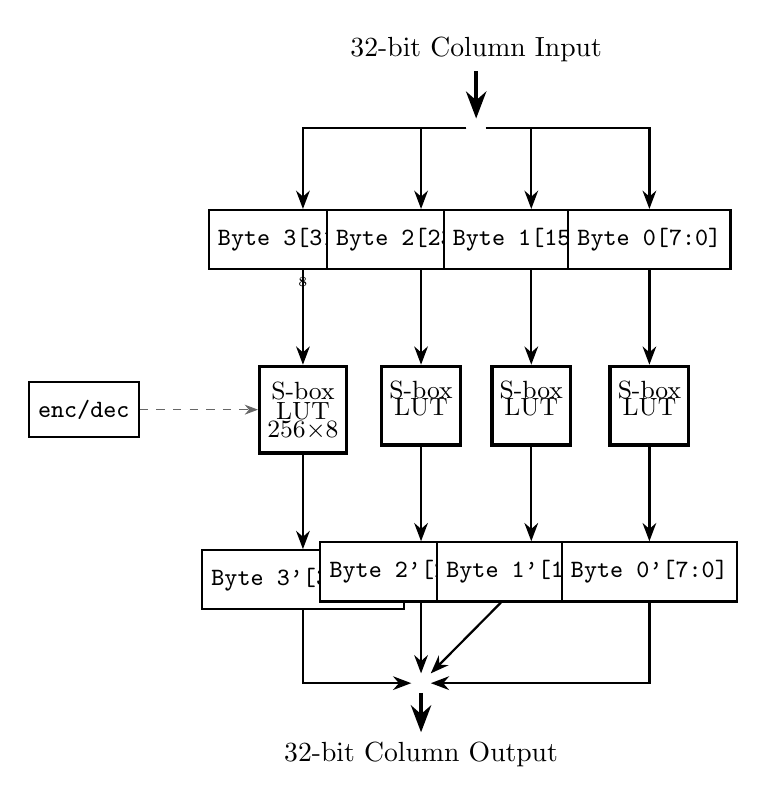
\begin{tikzpicture}[node distance=0.9cm]

% Input
\node[font=\normalsize] (in) {32-bit Column Input};
\node[below=0.6cm of in] (split) {};

% Input byte registers
\node[register, below=0.9cm of split, xshift=-2.2cm] (b0) {Byte 3\\{[}31:24{]}};
\node[register, below=0.9cm of split, xshift=-0.7cm] (b1) {Byte 2\\{[}23:16{]}};
\node[register, below=0.9cm of split, xshift=0.7cm] (b2) {Byte 1\\{[}15:8{]}};
\node[register, below=0.9cm of split, xshift=2.2cm] (b3) {Byte 0\\{[}7:0{]}};

\node[buswidth, below=0.05cm of b0.south] {8};

\draw[bus] (in) -- (split);
\draw[wire] (split) -| (b0);
\draw[wire] (split) -| (b1);
\draw[wire] (split) -| (b2);
\draw[wire] (split) -| (b3);

% S-box LUTs
\node[memory, below=1.2cm of b0] (sb0) {};
\node[font=\small, below=0.1cm of sb0.north] {S-box};
\node[font=\small, below=0.35cm of sb0.north] {LUT};
\node[font=\small, below=0.6cm of sb0.north] {256$\times$8};

\node[memory, below=1.2cm of b1, minimum width=1cm, minimum height=1cm] (sb1) {};
\node[font=\small, below=0.08cm of sb1.north] {S-box};
\node[font=\small, below=0.3cm of sb1.north] {LUT};

\node[memory, below=1.2cm of b2, minimum width=1cm, minimum height=1cm] (sb2) {};
\node[font=\small, below=0.08cm of sb2.north] {S-box};
\node[font=\small, below=0.3cm of sb2.north] {LUT};

\node[memory, below=1.2cm of b3, minimum width=1cm, minimum height=1cm] (sb3) {};
\node[font=\small, below=0.08cm of sb3.north] {S-box};
\node[font=\small, below=0.3cm of sb3.north] {LUT};

\draw[wire] (b0) -- (sb0);
\draw[wire] (b1) -- (sb1);
\draw[wire] (b2) -- (sb2);
\draw[wire] (b3) -- (sb3);

% Output byte registers
\node[register, below=1.2cm of sb0] (o0) {Byte 3'\\{[}31:24{]}};
\node[register, below=1.2cm of sb1] (o1) {Byte 2'\\{[}23:16{]}};
\node[register, below=1.2cm of sb2] (o2) {Byte 1'\\{[}15:8{]}};
\node[register, below=1.2cm of sb3] (o3) {Byte 0'\\{[}7:0{]}};

\draw[wire] (sb0) -- (o0);
\draw[wire] (sb1) -- (o1);
\draw[wire] (sb2) -- (o2);
\draw[wire] (sb3) -- (o3);

% Merge point
\node[below=0.9cm of o1] (merge) {};
\node[font=\normalsize, below=0.5cm of merge] (out) {32-bit Column Output};

\draw[wire] (o0) |- (merge);
\draw[wire] (o1) -- (merge);
\draw[wire] (o2) -- (merge);
\draw[wire] (o3) |- (merge);
\draw[bus] (merge) -- (out);

% Mode control
\node[register, left=1.5cm of sb0, minimum width=1cm, minimum height=0.7cm] (mode) {enc/dec};
\draw[controlwire] (mode) -- (sb0.west);

\end{tikzpicture}
\end{document}
